%%% Time-stamp: <mainrep.tex 19:57, 17 Jul 2016 by P Sunthar>
%%% $Log:$
% This document describes how to use iitbreport style
%********************************************************************

%\documentclass[11pt,a4paper,openright]{report}
\documentclass[openany]{iitbreport}
\linespread{1.25}	
%% Default spacing: 1.5
%% Default font size: 12pt
%% Default font: txfonts (similar to times new roman) 

%% Selectively comment out sections that you want to be left out but
%% maintaining the page numbers and other \ref
\includeonly{%
  intro/introduction,
  lit/literature,
  %expt/experimental,
  rnd/results, 
  dec,abs,pub,ack,nomen
}

%%% Some commonly used packages (make sure your LaTeX installation
%%% contains these packages, if not ask your senior to help installing
%%% the packages)

\usepackage{booktabs}
\graphicspath{{Pics/}}
%\usepackage{longtable}
%\usepackage{tabularx}
%\usepackage{rotating}
\usepackage{pdflscape}



%%% Macro definitions for Commonly used symbols
\newcommand{\Rey}{\ensuremath{\mathrm{Re}}}
\newcommand{\avg}[1]{\ensuremath{\overline{#1}}}
\newcommand{\tenpow}[1]{\ensuremath{\times 10^{#1}}}
\newcommand{\pder}[2]{\ensuremath{\frac{\partial#1}{\partial#2}}}

% Referencing macros
\newcommand{\Eqref}[1]{Equation~\eqref{#1}}
\newcommand{\Tabref}[1]{Table~\ref{#1}}
\newcommand{\Figref}[1]{Figure~\ref{#1}}
\newcommand{\Appref}[1]{Appendix~\ref{#1}}



\begin{document}
	
%%********************************Frontmatter***********************
% In frontmatter everything comes with roman numbering	
\pagenumbering{roman}
\setcounter{page}{1}

%*******************************************************************
%                         Title Page                            
%*******************************************************************
\title{Microgrid Reconfiguration}
\author{Sushrut D. Thakar}

%% Print the date. Today's date comes by default, change it here to 
%% other date format, if required:

%\date{\today}
\date{Jul 2016}


%% The type of the report can be set here

%\reporttype{A Seminar Report}
%\reporttype{A Thesis}
%\reporttype{A Dissertation}
\reporttype{Zeroth Stage Report}

%% Name of the degree
%\degree{EN 406}
\degree{Master of Technology}


%% Department/Centre Name
\dept{Department of Energy Science and Engineering}

%% Supervisor and cosupervisor/excosupervisor name can be put here
\supervisor{Prof. Suryanarayana Doolla}
%\cosupervisor{Cosper name}
%\excosupervisor{External Supervisor}

%% Roll number
\rollnum{Roll No. 13D170013}

\maketitle

%*******************************************************************
%                         Copyright Page                          
%******************************************************************* 
%\mycopyright                    

%*******************************************************************
%                         Dedication Page                         
%*******************************************************************
%\dedication[Dedicated to \ldots]        
%\addintoc{Dedication}

%*******************************************************************
%                        Certificate Page                         
%*******************************************************************
%\makecertificate[change title name]{report type} 
%\makecertificate{seminar report} 
%\makecertificate{thesis}
%\makecertificate{dissertation}
%\makecertificate{project report}

%\addintoc{Certificate}

%*******************************************************************
%                         Approval Sheet                         
%*******************************************************************
%\makeapproval{thesis}
%\makeapproval{dissertation}

%*******************************************************************
%                          Declaration                           
%*******************************************************************
%%==================================dec.tex================================
%
\begin{Declaration}
\noindent
I declare that this written submission represents my ideas in my own words and where others' ideas or words have been included, I have adequately cited and referenced the original sources. I declare that I have properly and accurately acknowledged all sources used in the production of this report. I also declare that I have adhered to all principles of academic honesty and integrity and have not misrepresented or fabricated or falsified any idea/data/fact/source in my submission. I understand that any violation of the above will be a cause for disciplinary action by the Institute and can also evoke penal action from the sources which have thus not been properly cited or from whom proper permission has not been taken when needed.

%
%
%
%
%
%
%

\DecSign[\today]



%
\end{Declaration}
%========================================================================
















 
%\addintoc{Declaration}

%******************************************************************
%                          Abstract                             
%******************************************************************  
%============================= abs.tex================================
\begin{Abstract}
This stage zero report on the topic of microgrid reconfiguration begins by presenting general concepts about microgrids and what reconfiguration means. Then a review of microgrid reconfiguration follows, in which various objective functions, constraints, methods and other considerations regarding microgrid reconfiguration as an optimization problem is presented. Finally some challenges for microgrid reconfiguration are noted and future work is discussed.
%
%
%
%
%
\end{Abstract}
%=======================================================================

                    

%******************************************************************
%                         Contents list                         
%******************************************************************
%\figurespagefalse
%\tablespagefalse
\makecontents % Creats toc, lof, and lot

%******************************************************************
%                        Notations                              
%******************************************************************
\notations[4cm]{List of Symbols and Acronyms}  
\nmA[]{CIGR\'{E}}{The International Council on Large Electric Systems (in French: Conseil International des Grands R\'{e}seaux \'{E}lectriques)}
\nmA[]{DSM}{Demand Side Management}
\nmA[]{PCC}{Point of Common Coupling}
\nmA[]{DER}{Distributed Energy Resource}
\nmA[]{PI Controller}{Proportional - Integral Controller}
\nmR[]{$P$}{Real Power}
\nmR[]{$Q$}{Reactive Power}
\nmR[]{$f$}{System Frequency}
\nmR[]{$V$}{Voltage Magnitude}
\nmA[]{VSI}{Voltage Stability Index}
\nmA[]{EV}{Electric Vehicle}
\nmA[]{NSGA 2}{Nondominated Sorting Genetic Algorithm - II}
\nmA[]{GA}{Genetic Algorithm}
\nmA[]{PSO}{Particle Swarm Algotrithm}
\nmA[]{AIS}{Artificial Immune System}
\nmA[]{V-AIS}{Vaccine-Enhanced Artificial Immune System}
\nmA[]{ICBA}{Improved Cellular Bat Algorithm}
\nmA[]{LP}{Linear Programming}
\nmA[]{APO}{Artificial Physics Optimization}
\nmA[]{SV-APO}{Search Vector Artificial Physics Optimization}
\nmA[]{AMOHSA}{Adaptive Multi Objective Harmony Search Algorithm}
\nmA[]{SAMCSA}{Self Adaptive Modified Clonal Selection Algorithm}
\nmR[]{$I_j$}{Current through $j_{th}$ line/branch}
\nmR[]{$Z_j$}{Impedance of $j_{th}$ line/branch}
\nmG[]{$\xi_L$}{The set of all the lines in the system}
\nmR[]{$t$}{Time Period selected}
\nmR[]{$R_j$}{Resistance of $j_{th}$ line/branch}
\nmR[]{$C_X$}{Cost of/Cost corresponding to X}
\nmG[]{$\xi_{DG}$}{The set of all buses with distributed generators (which are dispatchable)}
\nmA[]{DG}{Distributed Generator}
\nmA[]{PV}{Photovoltaic}
\nmG[]{$\alpha_j$}{The coefficient of $j^{th}$ line/branch which relates current flown to the maintenance and security costs}
\nmG[]{$\xi_D$}{The set of buses with shedable loads}
\nmR[]{$w_j$}{Weight assigned to $j^{th}$ element}
\nmR[]{$L_j$}{Load at $j^{th}$ bus}
\nmR[]{$G_k$}{The set of configurations which are radial and compatible}
\nmR[]{$N_X$}{Number of X}
\nmR[]{$x_j$}{The decision variable corresponding to switch status, is 0 if switch is open and 1 if switch is closed}
\nmG[]{$\xi_R$}{The set of lines/branches taking part in reconfiguration}
\nmR[]{$E_t$}{Energy Stored at time $t$}
\nmG[]{$\eta^{ch/disch}$}{Charging and discharging efficiency of the storage device}
\nmA[]{ENS}{Energy Not Supplied}
\nmA[]{SAIFI}{System Average Interruption Frequency Index}
%c\printnomenclature

%%********************************Mainmatter***********************
% In mainmatter everything comes with arabic numbering	
\cleardoublepage
\setcounter{page}{1}
\pagenumbering{arabic}

%******************************************************************
%                         Chapters                           
%****************************************************************** 
\newcommand{\etas}{\ensuremath{\eta_{\mathrm{s}}}}


\chapter{Introduction}


%\section{Microgrid in Background/Perspective}
%\section{What is Microgrid}
In simple terms, a microgrid is a power grid, but on a scale much smaller compared to conventional grid with its distribution system. 
Microgrid usually consists of a small system (distributed system, as opposed to centralized system which we have in place for our main grid.) , complete with its loads (of which there may be some vital loads which must be fed, and other non-vital loads) and some kind of generation capacity. This generation can be conventional - fossil fuel based, like using a microturbine, but ever more increasingly nowadays, also includes generation from renewables like wind and photovoltaics. There may be several other components according to the purpose of the microgrid, and some examples could be batteries and other storage devices, even electric vehicles, other kind of electricity generation systems like fuel cells, tidal energy etc. There may be some new technologies incorporated, like demand response and smart communications etc., and much more relevant to this seminar topic, switches which can cut some lines off/join those with the remaining microgrid (say sectionalizing and tie switches).

%defn given
 
The definition for the microgrid is given as ``A microgrid is a group of interconnected loads and distributed energy resources within clearly defined electrical boundaries that acts as a single controllable entity with respect to the grid. A microgrid can connect and disconnect from the grid to enable it to operate in both grid-connected or island-mode." by U.S. Department of Energy Microgrid Exchange Group\citep{TON201284} and ``Microgrids are electricity distribution systems containing loads and distributed energy resources, (such as distributed generators, storage devices, or controllable loads) that can be operated in a controlled, coordinated way either while connected to the main power network or while islanded." by CIGR\'{E} C6.22 Working Group\citep{CIGRE}.\\
%[https://building-microgrid.lbl.gov/microgrid-definitions]
%explanation (from old report maybe)
Note that there are loads as well as distributed energy resources (conventional or renewable) which can supply at least partly the loads. Due to this aspect, the microgrid is able to island. The U.S. Department of Energy Microgrid Exchange Group definition mentions that the microgrid acts as a single entity with respect to the grid, which just means that the grid only sees the power extracted by the microgrid through the point of common coupling between the main grid / distribution system and the microgrid, and the distribution system operator doesn't have to worry about what is going inside the microgrid, for such operator, microgrid is only a single aggregated load (or if the microgrid is injecting power into the main grid, a source or a negative load). The microgrid operator has to manage the microgrid, dispatching the distributed energy resources in the microgrid, as well as controlling other smart technologies inbuilt in the microgrid, like DSM( Demand Side Management) or reconfiguration etc. The topology/structure will be something like given in figure ~\ref{fig:certs1}. We can see that the microgrid is connected to the main grid via a static switch and PCC (Point of common coupling), so it can be disconnected from the main grid by opening that switch. Another feature we can see is that there are distributed energy resources which can partially/fully feed the loads.
\begin{figure}[tbp]
  \centering
    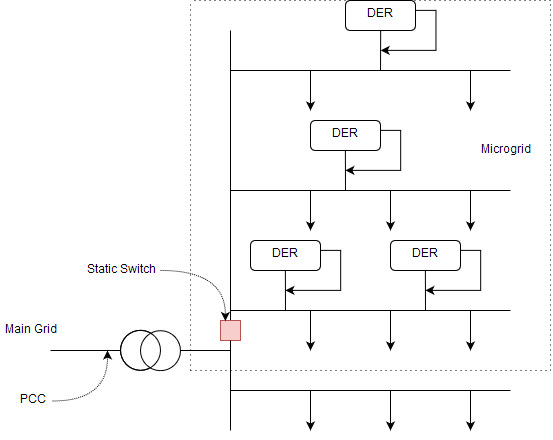
\includegraphics[width=1\textwidth]{MG_Illu.jpg}%paper1gridpaper1grid
    \caption[Microgrid Topology]{An illustrative microgrid topology}
    \label{fig:certs1} 
\end{figure}
%[1.1 of CERTS report]

%control of microgrids - variouslevels, description of each in %certain amount of detail. plus image for the control structure
Now, due to these peculiarities in microgrid, there are certain complexities in the control of microgrid, particularly because it has to be able to operate in islanded mode, isolated from the main grid. This creates several problems. In conventional power systems, the inertia of the system is quite high, because most of the generators are synchronous/rotating machines with high inertia. So conventional power system can deal with power imbalances by using this inertia and see relatively less change in the electrical parameters like voltage magnitude and frequency. However, in microgrid, in islanded mode, power balance is a big issue, because such inertia is simply not there. Even though there are distributed energy resources, they are mostly connected to grid through a power electronic interface, which doesn't offer the inertia similar to a rotating machine, and even if there are a few rotating machines (generators) as the distributed energy resources, they are comparatively much smaller in size and have much lesser inertia compared to their larger counterparts used in the main grids. Apart from acting similar to a slack for microgrid (which makes up for the imbalance of power), the main grid also provides voltage phase frequency and magnitude reference for the microgrid devices and can be generally relied upon to maintain these within specified limits, and there is no requirement of distributed energy resources having to also regulate the voltage magnitude, frequency, etc. This is not the case in islanded mode, however, and finding a control method which will ensure that the voltage magnitude and frequency is within limit is challenging, because the DERs(Distributed Energy Resources), by themselves usually do not have enough inertia to soak up the difference between the desired and actual values as a single DER, and coordinating the control just makes the control system difficult. For example, if we put a PI controller to control the voltage magnitude on two separate DERs, then we may see oscillations due to the competing control. There are usually two options suggested to deal with this. First is to have a decentralized control where a communication system is not needed. This includes having droop control, which doesn't rely on remote measurements and only requires local measurements, eliminating the need for communication between controllers. Most DERs, which are not rotating machines, can be represented by an inverter with filter at the output to suppress high frequency components generated due to switching action (figure~\ref{fig:certs31}).
\begin{figure}[tbp]
  \centering
    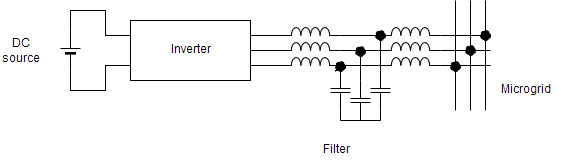
\includegraphics[width=1\textwidth]{DER-inv.jpg}%paper1gridpaper1grid
    \caption[DERs]{A DER connected via inverter to the microgrid}
    \label{fig:certs31} 
\end{figure}
The droop control is generally used in these DERs, and 
%(given in figure ~\ref{fig:certs32})
% \begin{figure}[tbp]
%   \centering
%     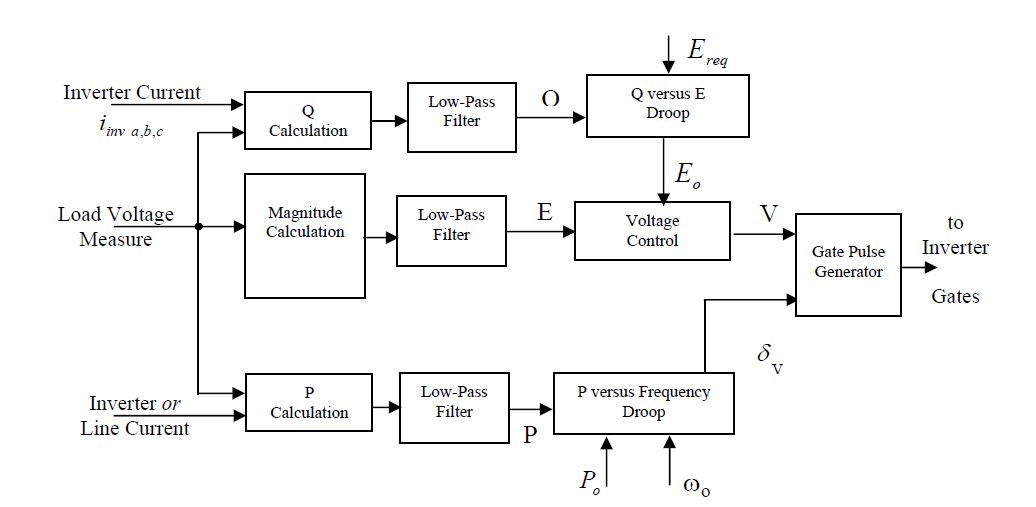
\includegraphics[width=1\textwidth]{certs32.JPG}%paper1gridpaper1grid
%     \caption[Control of DER]{Droop Control of a DER: Control Blocks(image adopted from \cite{CERTS-con})}
%     \label{fig:certs32} 
% \end{figure}
includes $P-f$ and $Q-V$ droops in each of the DERs, and each DER accordingly takes up some of the imbalance of power, resulting in voltage magnitude/frequency deviation. The droop curves (figure ~\ref{fig:00993176})
\begin{figure}[tbp]
  \centering
    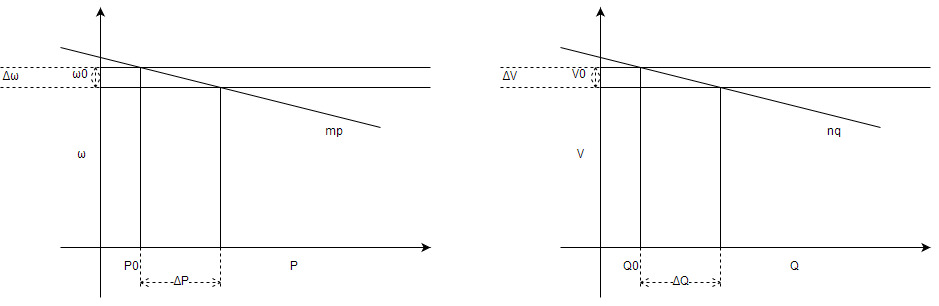
\includegraphics[width=1\textwidth]{Droop_Curves.jpg}%paper1gridpaper1grid
    \caption[Droop Curves]{$P-f$ and $Q-V$ Droop Curves}
    \label{fig:00993176} 
\end{figure}
can give an idea about how droop control works. When the frequency is below the setpoint, according to the droop curve, the real power generation increases, and this helps in bringing the frequency back up, and similarly for the other case and $Q-V$ droop. Now this works very well for real power - frequency droop, but not as much for the $Q-V$ droop, because the reactances of various lines and inductors in the system can cause detection of incorrect voltage levels, and there might be reactive power oscillating between sources. To eliminate this, sometimes a central controller controls all the DERs, loads etc, and gives a particular target to each DER, effectively sharing $P$ and $Q$ imbalance between the DERs. But a central controller requires higher processing power as well as a communication system between the central control system and all the DERs.
Another problem which microgrid operators may face when planning a dispatch etc. is that there is uncertainty in loads, but more importantly, the DERs, especially renewable DERs are quite uncertain, in a way that we can't control how much they generate and it depends on the available sunlight and wind, phenomena which can have very fast fluctuations. So the microgrid has to be able to deal with this uncertainty and absorb the difference via either control of dispatchable DERs, or balancing multiple renewable DERs, or having storage systems, etc.\\
%\section{What is Reconfiguration}	
%reasons for mg optimization - sustainability, efficiency, reliability
There are various reasons to operate a microgrid even though there are certain challenges. For one, it can absorb high amount of renewable DERs without the distribution or transmission system operator having to worry about the local issues. Also, it can be interfaced with many small scale DERs, and efficiently capture as much energy as possible. Due to its small scale, new technologies can easily be integrated into a microgrid, and the system can be operated very efficiently. Another reason to operate a microgrid is that a microgrid has its own DERs, so it is not entirely dependent on the main grid for its operation, and can survive faults and interruptions caused in/by the grid. This creates much more reliable system. These three - sustainability, efficiency, and reliability are why microgrids are used and also how they are operated/planned\citep{mgb05}.
%[refer to mgb 05 and rewrite, and cite it as well]
This usually includes an optimization in order to achieve either of/ some of/ all of these goals in some way.
%different tools available for microgrid optimization
In order to operate this microgrid efficiently and achieve these goals, the operators have various tools at their disposal. These include power exchanged with the main grid, dispatchable DERs, dispatchable loads, storage systems, reconfiguration, and some more depending on the particular cases. Power exchanged with the main grid is unavailable during islanding. While PV (Solar photovoltaic) and wind are generally not considered dispatchable, and we want to utilize maximum energy out of them, other DERs can be dispatchable, such as micro-hydro-turbines, small generators running on fossil fuels, fuel cells, etc. The real as well as reactive power fed by them can be controlled up to a point. Dispatchable loads and DSM can be used to modify the loads or the demand of the system, thus balancing the power generated with the power used, and making the microgrid operation more economical. These schemes may include direct control of the loads by the microgrid operator, or some incentive based scheme where the users are given an option and incentives to perform a certain action. Storage devices can be controlled as well, by controlling their charging-discharging, and there are various options for storage as well.\\
%what is reconfiguration - general idea
Reconfiguration means that we change the network topology itself, not only a-priory but \textit{while} the microgrid is operating as well (\citep{mgrrev01}). Reconfiguration in microgrid is possible due to a large number of lines in microgrids which are tie switches or sectionalizing switches. This can be used in addition to the conventional control variables to achieve better efficiency, lesser costs, lesser losses, more number of loads fed, or any other objective one might want the microgrid to achieve.
%devices involved/operation
This reconfiguration requires presence of tie (normally open) and sectionalizing (normally closed) switches. These enable the microgrid operator to open and close certain lines in the system. The switches can be automatically operated, working on the instructions of the central controller (if such controller exists) or can be operated manually.
%illustrative example
This example provided in \citep{mgrj18} is a very good illustrative example while explaining how reconfiguration takes place (see figure ~\ref{fig:khav1}).
\begin{figure}[tbp]
  \centering
    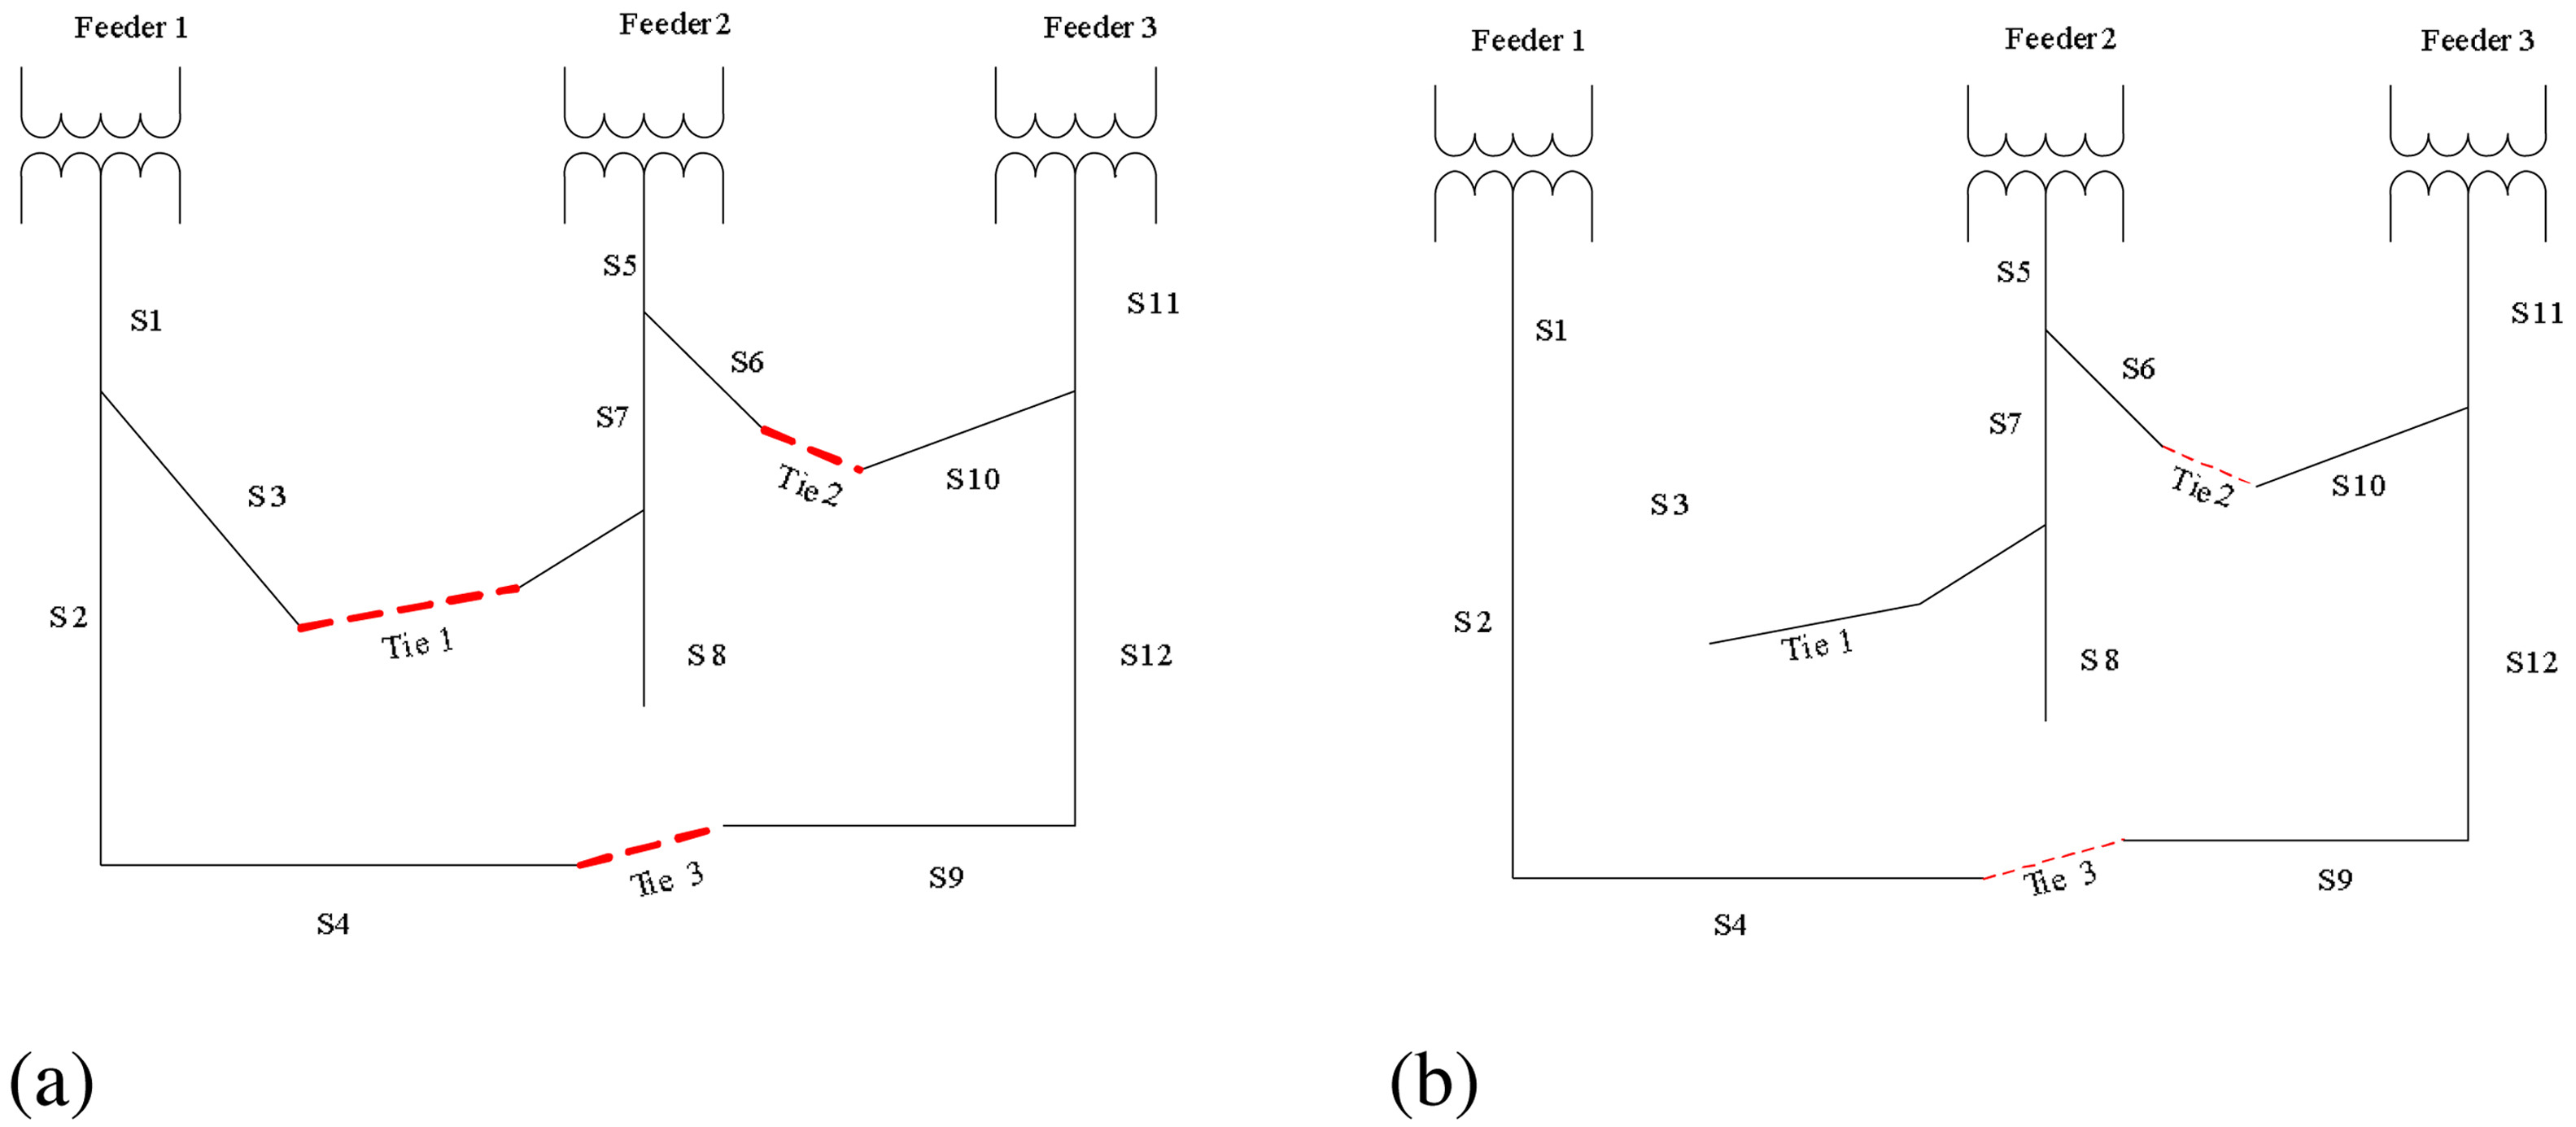
\includegraphics[width=1\textwidth]{khav1.jpg}%paper1gridpaper1grid
    \caption[Reconfiguration]{An illustrative example of reconfiguration(\citep{mgrj18})}
    \label{fig:khav1} 
\end{figure}
In case (a) shown, the initial system is presented. The dotted lines indicate open switches. Now suppose feeder 1 is nearly loaded to its full capacity, and feeder two is quite underloaded, then we might want to shift a load or two on feeder two from feeder 1. We can do this by closing Tie 1 switch and opening S3 switch. Now the load on feeder 1 is a little bit lesser than before, and feeder 2 is a bit more loaded than before. Here the objective was to decrease the load on feeder 1, and since it was a small system with no generation, no PCC to be able to island etc. we could simply choose what to do. As complexity of system increases, choosing when and which switches to operate and which configuration to attain can be quite complicated, but the idea behind reconfiguration is the same.\\
The remaining report presents an exhaustive literature review on the reconfiguration of microgrids, and classifies it, in the chapter ~\ref{ch2}, and concludes in ~\ref{ch4} by stating some of the challenges and future work in the area of microgrid reconfiguration.

%%


%%% Local Variables: 
%%% mode: latex
%%% TeX-master: "../mainrep"
%%% End: 

\chapter{Literature Survey} \label{ch2}
In this chapter a brief discussion of work done by various researchers in this area for the last two decades is presented. Balaji and Venkateshan\citep{BALAJI1993260} have developed a model to investigate the significance of radiation in natural convection inside a square cavity. Even though their work does not discuss solar applications, it has shown light to heat loss mechanisms that are taking place in a cavity. Work of Balaji and Venkateshan [12] can be considered as the first proper attempt to prove the effect of radiation in free convection cavity problems. For convection, Boussinesq approximation has been used for simplification of the governing equations. They have developed a correlation to obtain radiation and convection Nusselt number. They have also shed light on "dual nature" of radiation. The increase in radiation causes convection Nusselt number to drop while overall Nusselt number which is the combination of both radiation and convection Nusselt numbers can either increase or decrease depending on other factors like emissivity of walls, temperature ratio etc. Pye et. al.\cite{pye2003modelling} modeled a simple trapezoidal cavity with emissivity and temperature values close to the actual values of the experiment. They assumed a constant temperature for the absorber. The simulation was done in Fluent 6.0 for different cavity depth, cavity width, the temperature of absorber plate, ambient temperature and convection coefficient of outer surface the glass covering. For convection, Boussinesq approximation is used and Discrete Transfer Model for radiation (DTRM) is used. Grid size used was $2\ mm$ where triangular grids used in the side walls and rest square grids are used. They have depicted heat flow process from absorber as described further. Absorber receives solar radiation and its temperature rises. Other surfaces of cavity receive heat from absorber through a combination of conduction, convection and radiation. Heat energy then gets conducted to external surfaces of the cavity receiver. Then through a combine effect of convection and radiation, it escapes the cavity. Radiation dominates the internal heat transfer process because absorber temperature is very high and heat transfer through radiation is proportional to differences in the fourth power of surface temperatures. Convection contributes only 8\% of total heat transfer inside the cavity. Convection dominates in heat transfer exchange between the outer surface of the cavity and surroundings. Because the glass, through which heat is mainly transferred to the atmosphere; is not at that high temperature from the outside air They also found that the top space of the cavity is almost stratified so that only conduction is present and at the bottom part convection is present at very
low velocity which explains the low convection percentage in the losses. They proposed relations for external as well as internal radiation and convection losses. They fixed all non-dimensional parameters like emissivity and external heat transfer coefficient and varied only depth and width of the cavity. Other non-dimensional parameters are found for the air temperature inside the cavity (approximated by taking an average of glass cover temperature and
absorber tube temperature. The relation given by them for the convective Nusselt number inside the cavity is as follows.
\begin{equation}
Nu_{conv} = 1.1917(Gr)^{.10363}(D/W)^{.6432}
\end{equation}
For internal radiation losses, they proposed simple parallel plate formula and for external
radiation and convection losses; normal convection radiation formulas for a plate at constant
temperature is proposed.

Singh et. al.\citep{SINGH2010329} introduced different shapes and coatings for the absorber. Their studies were completely experimental. They used a single square shaped absorber as well as six round absorber pipes in the trapezoidal cavity. They combined normal coating and selective coating in them and studied the changes in thermal performance. They also introduced a double glass cover since most of the losses are occurring through the glass cover. They passed oil through the absorber and found out the heat loss from entry to exit and equated it to the heat loss taking place from the absorber to the other components, thus obtained the heat transfer coefficient. They also the selective coating offered 20-30\% less heat transfer coefficient compared to the ordinary black paint. The use of double glass covers of the cavity offered a 10-15\% lower heat transfer coefficients for different absorber temperature. They developed a correlation between heat transfer coefficient and absorber temperature. They also found out the values analytically by using correlation obtained by Balaji and Venkateshan\citep{BALAJI1994249} and correlation for heat transfer coefficient between parallel plates.
However, both showed a significant difference from the experimental values.
All of these CFD models were able to show the flow patterns correctly. However, the losses predicted showed a significant variation. Reynolds et. al.\citep{REYNOLDS2004229} predictions using CFD model showed excellent agreement with actual flow pattern. They compared their simulation result using Fluent 5.0 with the experimental results. They observed the same pattern in the simulated model and experimental model which can be seen in fig.\ref{rey}. 

\begin{figure}[H]
\begin{center}
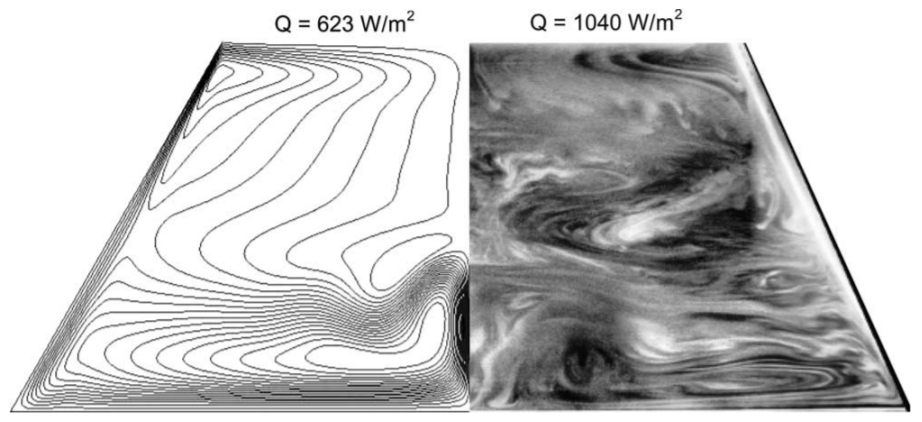
\includegraphics[width=\textwidth]{reynolds40.PNG}
\caption{Comparison between CFD simulated from pattern
(left) to the experimentally observed pattern obtained by
Reynolds et. al.\citep{REYNOLDS2004229}}
\label{rey}
\end{center}
\end{figure}

They also observed that the 2/3rd of the cavity in the top is thermally stratified and the remaining part of the cavity has counter-rotating flows on either side of the symmetry plane. Even though their flow pattern is in excellent agreement with the CFD simulated model, the CFD model under predicted the losses by more than 40\%. Their explanation was that it is because of the uncertainties in measurement. At this point Fac\~ao and Oliveira\citep{FACAO201190} used a new model where the absorber is modeled as a lower half of the pipes with no gap as shown in the Fig.\ref{facao}

\begin{figure}[H]
\begin{center}
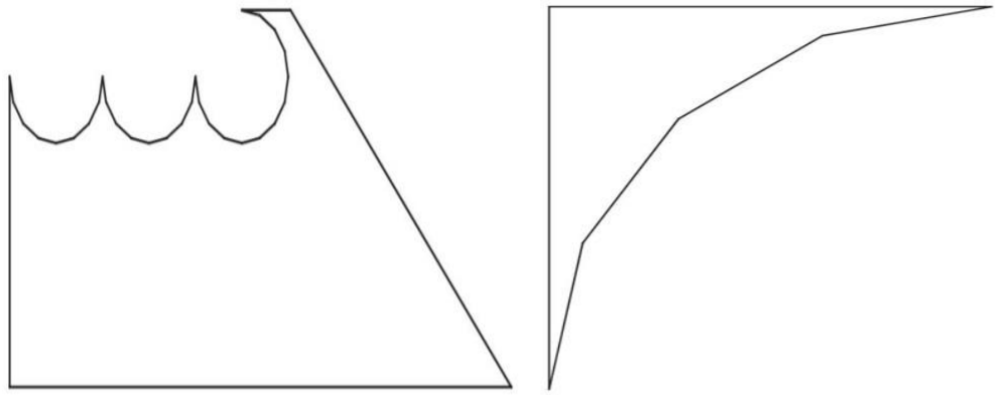
\includegraphics[width =\textwidth]{faco.PNG}
\caption{Modified model of trapezoidal cavity including the pipes (left) Circular cross-section of pipe approximated
as hexadecagons for easy meshing and faster convergence (Right) proposed by Pye et. al.\citep{pye2003modelling}}
\label{facao}
\end{center}
\end{figure}

Initially, this model is proposed by Pye in his Ph.D. thesis\citep{pye2008system}. Pye et. al.\citep{pye2003modelling} simulated heat losses in the cavity using Fluent and found that radiation losses are 25\% higher than the value obtained when an isothermal flat surface is used. Therefore, they concluded that geometry of the pipe does matter in heat loss analysis. Fac\~ao and Oliveira\citep{FACAO201190} took this observation and approximated lower half circle as regular hexadecagons as shown in Fig.\ref{facao} to avoid convergence issues and inaccuracies. They changed two geometric parameters which are the depth of the cavity and insulation thickness of sidewall. Also, they considered two different heat transfer coefficients for the external side of the glass cover to accommodate two different wind velocities. Total eighteen sets of simulations are carried out using combinations of these parameters. They compared the heat transfer coefficients obtained with the other available literature and found that their values are significantly higher; that means closer to the experimental values and hence showed the importance of inclusion of geometry of the pipes. Different values thickness of insulation and depth of cavity were used in their simulation to find out heat transfer coefficient and choose the best thickness and depth by trial and error. Flow pattern obtained by him for the modified geometry is shown in Fig.\ref{facaoresult}

\begin{figure}[H]
\begin{center}
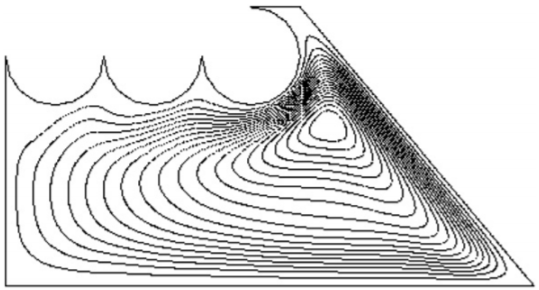
\includegraphics[width=\textwidth]{facoresult.PNG}
\caption{ Stream lines obtained in model with modified geometry by Fac\~ao and Oliveira\citep{FACAO201190}}
\end{center}
\label{facaoresult}
\end{figure}


Later, Sahoo et. al.\citep{SAHOO201318} modeled full absorber pipes of certain numbers with gaps between them. They validated their result with experimental models and then analyzed the effect of various parameters such as receiver tube surface temperature, receiver depth, the number of tubes, and emissivity of the outer surface of the receiver tubes. They have concluded that contribution of convection is between 5\% and 18\% of the total heat losses. They got an excellent agreement between the simulated results and the experimental heat transfer values except at high temperatures. Their explanation was that it is because of the approximation that top of the cavity is completely insulated and heat loss from it was neglected. They compared the obtained heat transfer coefficient values with the results by Fac\~ao and Oliveira\citep{FACAO201190} and Pye et. al.\citep{pye2003modelling}. They got an increase of 24-29\% increase with respect to Pye et. al.\textquotesingle s values and 4-13\% increase with respect to Fac\~ao and Oliveira\textquotesingle s values. The obtained temperature contour is shown in fig.\ref{sahooresult}

\begin{figure}[H]
\begin{center}
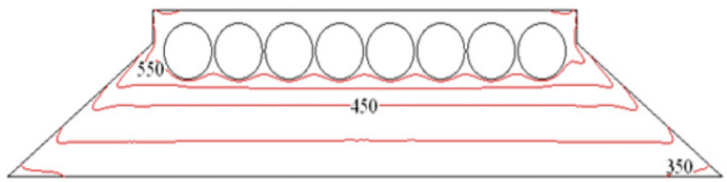
\includegraphics[width=\textwidth]{sahooresult.PNG}
\caption{Isotherms obtained by Sahoo et. al. for 8 pipes with gap\citep{SAHOO201318}}
\end{center}
\label{sahooresult}
\end{figure}

Natarajan et. al.\citep{NATARAJAN2012523} again assumed the flat absorber top for their CFD simulations but did not use Boussinesq approximation. They have solved 2-D geometry with laminar and steady-state condition using implicit solver. For changes in viscosity, it calculated by using Sutherland\textquotesingle s theory of viscosity with three coefficient method. They made a point that Boussinesq approximation is not valid for temperature above $100^0\ C$ which is the case at the top part of the cavity. They studied heat losses by varying aspect ratio, temperature ratio, Grashof number, surface emissivity, absorber angle and radiation conduction number. As per their observation, increasing the aspect ratio causes increment in the thickness of the static air region near the upper part of the cavity which reduces the overall loss of heat in a trapezoidal cavity. The increment in temperature ratio causes increased difference in temperature between the top wall and the bottom wall of the cavity but has negligible effect on the thickness of static air zone. However, it reduces heat transaction between top and bottom wall but this decrement becomes sluggish beyond certain temperature ratio($T_c/T_h$) equal to $0.6$. Thus, in general, heat loss in a trapezoidal cavity can be reduce to a certain extent by increasing aspect ratio and temperature ratio. Moghimi et. al.\citep{MOGHIMI2015343} modeled a full cavity with insulations and used CFD tools to optimize the cavity design to minimize the losses as well as to get desired wind resistance. They have used discreet ordinate (DO) method to include the semi-transparent properties of glass. From the
temperature patterns they have observed that below the pipes; radiation and conduction heat transfer dominates as can be seen from fig.\ref{optz}.

\begin{figure}[H]
\begin{center}
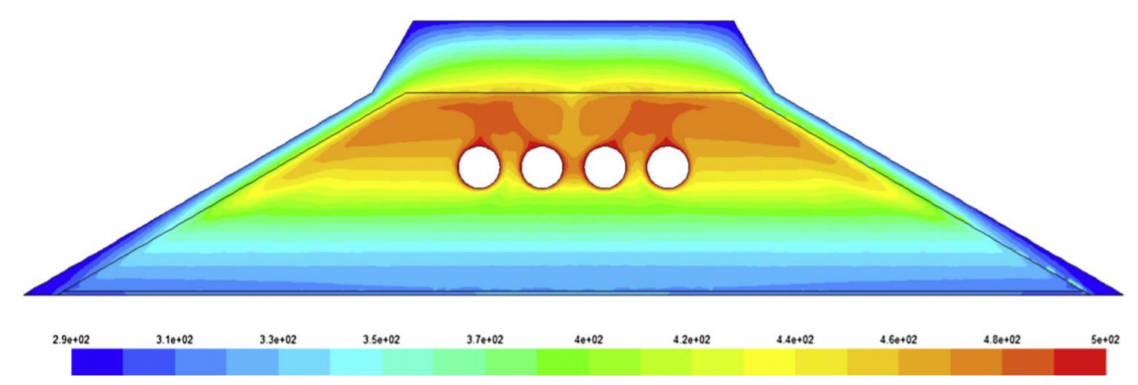
\includegraphics[width=\textwidth]{optz.PNG}
\caption{Temperature contour obtained by Moghimi et. al.\citep{MOGHIMI2015343}}
\end{center}
\label{optz}
\end{figure}

All the research work until this point have been done by solving Navier-Stokes equation for convection. But convection consists of two heat transfer methods namely conduction and advection. Mohan et.al. \citep{MOHAN201837} have shown that conduction accounts for more than 99\% of heat transfer by convection. To prove this they have shown two studies on trapezoidal cavity receiver. First study shows comparison of heat transfer using convection against heat transfer using conduction only in TCR. Obtained results show remarkable similarity. Second study shows comparison of heat transfer using convection+radiation against heat transfer using conduction+radiation. Again in this study results obtained from both the methods are quite close. Obtained Nusselt number at the hot in both the cases is within 1\% of each other which can be seen in the following table \ref{tab:sarathcomptable}. This study shows that even if we take conduction and radiation as heat transfer method in a TCR, same results can be achieved as with convection and radiation as extent of advection is quite insignificant. This also gives an advantage by reducing complexity of the model as Navier-Stokes equation has no longer to be solved.

\begin{table}[H]
\centering
\caption{Heat flux and Nusselt number of hot wall in a trapezoidal cavity}
\label{tab:sarathcomptable}
\begin{tabular}{|c|c|c|l|l|}
\hline
\textit{\textbf{At the hot wall}} & \textbf{Convection} & \textbf{Conduction} & \textbf{\begin{tabular}[c]{@{}l@{}}Convection+\\ Radiation\end{tabular}} & \textbf{\begin{tabular}[c]{@{}l@{}}conduction+\\ Radiation\end{tabular}} \\ \hline
Total heat (W)                    & 50.06               & 49.00               & 899.90                        & 892.27                        \\ \hline
Total radiation heat (W)          & 0.00                   & 0.00                   & 845.96                        & 846.99                        \\ \hline
Nusselt number                    & 1.12                & 1.10                & 20.24                         & 20.07                         \\ \hline
\end{tabular}
\end{table}














%\chapter{Microgrid Reconfiguration in Action: Selected Applications} \label{ch3}

\section{Reconfiguration in Microgrid Combined with Unit Commitment }\label{ch3sec1}
This section will explain how use of reconfiguration in microgrids can be useful while solving a unit comittment problem in microgrid in order to further enhance it , and is mainly based on ``Microgrid operation and management using probabilistic reconfiguration and unit commitment" by ``Reza Jabbari-Sabet , Seyed-Masoud Moghaddas-Tafreshi, Seyed-Sattar Mirhoseini"\citep{Jabbari-Sabet2016328}. This paper was published in International Journal of Electrical Power \&  Energy Systems in February 2016. This paper is combining unit comittment and microgrid reconfiguration, or in other words, enhancing unit comittment problem in microgrids by allowing microgrid reconfiguration. They look at a day-ahead unit comittment problem from the perspective of microgrid manager, and try to find optimum unit commitment and optimum network topology (via reconfiguration) so as to maximize benefit or profit which the micogrid manager makes. Authors optimize this system for several cases, considering wind input to be probabilistic in nature, and then aggregate the results.\\
\subsubsection{Problem Formulation and Assumptions}
The benefit or profit can be written for the day ahead problem as
\begin{eqnarray}
Max: OF = \sum\limits_{t=1}^{24}(revenue(t)-cost(t))
\end{eqnarray}
The system selected in this paper is a 10 bus system, with 3 microturbines(MTs) (which run on conventional fossil fuels), 1 battery interfaced with an inverter, a wind generator, and this system is connected to grid through a single bus.(as shown in the Figure ~\ref{fig:pap1grid})
\begin{figure}[tbp]
  \centering
    \includegraphics[width=0.8\textwidth]{paper1grid.jpg}%paper1gridpaper1grid
    \caption[Paper 1 Microgrid System]{The microgrid model used for study in paper 1(image adopted from \cite{Jabbari-Sabet2016328})}
    \label{fig:pap1grid} 
\end{figure}

A total number of 8 loads are considered, with some of them being vital loads and others non vital. The authors try to perform this optimization by selecting their decision variables as all of the microturbine power outputs, the power exchanged with battery, the power exchanged with grid, and the network configuration (which essentially denotes which lines are open in the network, hence the network topology- several cases are given various numbers, and the variable $n\_topology$ stores that particular configuration number) for all the time periods, which results in a total of $24\times6=144$ decision variables, which includes 6 decision variables per hour (namely the power outputs of 3 MTs, the power exchange with battery, the power exchanged with grid, and the $n\_topology$ for that hour) for 24 hours.\\
In considering revenue and cost part of the objective function, the authors have included several sources of revenue and several components for cost: in the revenue part, the authors are considering two components: the revenue generated by feeding off the loads, and also the revenue generated through selling electricity to the grid (As can be seen in the equation ~\eqref{eq:pap1rev})
\begin{eqnarray}
\label{eq:pap1rev}	
revenue = R{load} + R{network}\\
R{load} = \sum\limits_{k=1}^{N_{load}}(\rho_{load,k}\cdot p_{load,k}\cdot t)\\
R_{network} = \rho_{sell-network}\cdot p_{sell-network}\cdotp t\\
\end{eqnarray}
where $\rho_{load,k}$ is the price of electricity for that time period for the $k^{th}$ in the microgrid, $p_{load,k}$ is the total load at the $k^{th}$ bus during the  interval, $t$ is equal to one hour (since the day ahead calculations are done hour by hour), $\rho_{sell-network}$ is the price at which microgrid can sell electric power to grid utility, and $ p_{sell-network}$ is the actual load the network sells to the grid during that hour. Note that all of these equations depict revenue generated in one period, and the revenue for each period can be calculated by using these equations. Note that both the prices are not fixed, so $\rho_{load,k}$ and $ \rho_{sell-network}$ vary according to the time of the day ($\rho_{buy-network}$ also varies according to the time of the day, but that will come in the costs). In addition, the vital and non vital loads buy electricity at different prices, with prices for vital loads being higher.\\
The costs include various costs: there are costs associated with power generation from all three microturbines as well as wind generator, the costs associated with buying power from the utility (grid), costs associated with power loss within the microgrid and the cost of switching (which comes into play because we might be reconfiguring the network, according to the optimization process). In equation form,
\begin{eqnarray}
\label{eq:pap1cost}
cost = \sum\limits_{j=1}^{N_{mt}}C_{mt}(j) + C_{wind} + C_{bat} + C_{network} + C_{loss} + C_{switching}
\end{eqnarray}
The above equation ~\eqref{eq:pap1cost} denotes the cost for one period. Total cost would be, then, the above expression summed over all of the intervals.
The models used for each of these costs are usually the standard ones: for microturbines, for instance, the cost is divided in terms of quadratic fuel cost, O\&M cost proportional to power output, startup cost (since this is a unit commitment problem), capital cost, and emission cost. While considering startup cost, it is considered that the startup cost increases as the microturbine is kept off for more and more time, the capital cost is given as annualized capital cost, and emission cost is considered to be proportional to the power generated.
The cost associated with wind power generation is calculated by calcutating two terms, O\&M term, which is taken constant (irrespective of the wind power generated), and capital cost, which is annualized. 
Battery cost also includes two terms, cost associated with the usage of battery, i.e. charging or discharging, which is proportional to the power battery exchanges with the microgrid for a period, which also includes a correction which accounts for battery degradation, i.e. cost increases as the battery gets older and has been used for more cycles, and second term which is O\&M cost, which is considered to be constant. 
Network cost is simply the amount of power bought from the utility for a particular interval times the price of the electricity. Note that the authors have not used a fixed price, but the price varies according to the time of the day. 
Switching cost is the result of the authors allowing reconfiguration of the system, and has two components, a capital cost, annualized, and another component which is proportional to the number of switching operations performed.\\
The constraints the authors have considered include standard constraints considered for unit comittment problem, i.e. the bus/node voltages should be in acceptable range, the currents should not exceed the line flow limits, the demand should be met inspite of losses (power balance), the generation limits for microturbine, the limits on battery power exchange, the limits on SOC of the battery, the limits on the grid power exchange etc. In addition, since this is a unit commitment problem, minimum uptime and downtime constraints are also added. Also, the topology constraint is added since this is a reconfiguration problem, which states that the network topology should always be radial (since this is a microgrid, akin to a distribution system).




\subsubsection{Methods}
When trying to solve this optimization problem, authors have considered the wind power output as well as load to be probabilistic and not deterministic, hence a probabilistic treatment to the problem is needed. The authors create multiple scenarios according to the probability distributions of wind speed and load, and solve a deterministic problem for each scenario. The results are then aggregated and analysed.\\
The wind turbine power depends on the wind speed and hence changes from scenario to scenario. For each period, 12 years' hourly wind speed data is available, and that is used to fit a Weibull distribution by relating the mean and standard deviation of the wind speed data to the parameters of Weibul distribution (equation~\eqref{eq:pap1wei}: here $r$ and $c$ are parameters of Weibull distribution dependent on the mean and variance of wind speed data).
\begin{equation}
\label{eq:pap1wei}
f(w) = \frac{r}{c}\left(\frac{w}{c}\right)^{r-1}\exp\left[-\left(\frac{w}{c}\right)^r\right]
\end{equation}
Then, for each scenario, a random number between 0 and 1 is generated for each hour, and on the Cumulative Distribution Function (CDF) of that hours' Weibul distribution, the value corresponding to CDF being that number is found and used as the wind speed for that particular hour. The wind power generated, then, is calculated by assuming quadratic dependence of power generated on the wind speed from cut in speed till the rated speed, and constant power output up to the cutoff speed after that. Loads are treated similarly, the only difference is that the probability distribution considered here is normal.\\
Once the wind power and load data is generated according to the scenario for each hour, it only remains to solve a deterministic unit comittment and reconfiguration problem, which is not necessarily an easy feat, due to presence of mixed integer programming required. The method employed in the paper by the authors is the particle swarm optimization (PSO). PSO technique is an evolutionary technique, which tries to search for a global optimum of a function. It starts by creating a set of random solutions within the allowed solution space, called particles. It then calculates the function value at all those solution points. Then it finds the particle best for each particle (this solution is the best function value it has reached so far- so for the first iteration, it will just be the function value) and the global best value- the best value any particle has reached so far (in the first iteration it will be the minimum value amongst the particles initiated). In the second phase it calculates a 'velocity' for each particle, which is calculated according to the difference between the value of the function at current position of a particle, and the particle best, and also the difference between the value of the function and the global best. Both these are multiplied by a random number between zero and one, and a weight given to each of these differences (usually equal weight is given- 2 for each term), and then these terms are added to current velocity in order to update it(equation ~\eqref{eq:pap1pso1}). Also the particle position is calulated according to the velocity(equation ~\eqref{eq:pap1pso2}), and hence each particle reaches at a new solution.
\begin{eqnarray}
\label{eq:pap1pso1}
v_{new} = v_{old} + c_1*r_1*(particle\_best - current) + c_2*r_2*(global\_best - current)
\end{eqnarray}
\begin{eqnarray}
\label{eq:pap1pso2}
position = position + velocity
\end{eqnarray}
In each new iteration, if applicable, particle best and global best value are updated, and those solutions are stored. Finally, when either maximum number of iterations are reached, or the particles reach a best solution and hence stop their movement, the method ends, and the gbest value and the corresponding solution are given as the output.
Generally, PSO is designed to work when we have an unconstrained optimization problem. Here though, there are many constraints which need to be satisfied, and hence if solution reached is violating any of the constraints (after calculating the losses  by doing forward/backward sweep load flow analysis), a penalty function is added to the objective function.\\
After calculating the optimum solution for the UC and reconfiguration problem for each scenario, such scenarios have to be aggregated to get an overall picture. This scenario aggregation is done using expected value. Also, coefficient of variance (which is standard deviation, relative to the mean) is computed, and if it is small, then the results are consistent. Since the topology code ($n_{topology}$) is a discrete variable, it is aggregated not by using expected value, but by taking the value which is seen the most i.e. taking the mode.
\subsubsection{Results and Discussion}
The authors find that there are two configurations of the network which are most commonly seen. It is seen that the MG sells electricity to the grid for most of the time, but buys near it's peak. The benefit by using this probabilistic reconfiguration and UC turns out to be 49,891 cents, with 3270 cents standard deviation. If only UC is used, 53,068 cents mean value for benefit is achieved, with standard deviation 13,863 cents. While it seems that the benefit achieved is less due to reconfiguration plus UC, where this method seems to be gaining is accuracy. The authors have done the calculations also on actual load and wind data for that particular date in 2012, and in both cases the benefit achieved turns out to be around 50,000 (50,691 in UC and reconfiguration, and 50,266 in case of only UC), so reconfiguration plus UC value is much more closer to reality and hence better prediction of real life situation. The authors have also varied the number of scenarios, and it turned out that at lower scenarios the coefficient of variation is higher, while it becomes low and converges when then number of scenarios get high, and is less than 1 percent when the number of scenarios is higher than 40.



\section{Electric Vehicles and Microgrid Reconfiguration}\label{ch3sec2}
This section explains how electric vehicles (EV) and reconfiguration can be integrated in order to benefit the microgrid by reducing the costs incurred, and is based on ``Efficient integration of plug-in electric vehicles via reconfigurable microgrids" by ``Abdollah Kavousi-Fard, Amin Khodaei"\citep{Kavousi-Fard2016653}. This paper was published in Energy in September 2016. This paper deals with microgrid reconfiguration from economic perspective, similar to previous paper, but considers presence of plug-in electric vehicles in addition to reconfiguration. The authors try to minimize the operating costs of running the microgrid and analyses the effects of reconfiguration and plug in electric vehicles on the overall cost of the microgrid. The analysis is done stochastically, by generating various scenarios and then solving the problem deterministically for each scenario. The authors have also considered the presence of various renewable generators while performing this analysis.
\subsubsection{Problem Formulation and Assumptions}
The system considered in this paper is a modified 32-bus IEEE system, with 1 PV source, 2 wind sources, 2 microturbines, 1 fuel cell, and two vehicular fleets(see figure ~\ref{fig:pap2grid}).
\begin{figure}[tbp]
  \centering
    \includegraphics[width=0.85\textwidth]{paper2grid.jpg}%paper1gridpaper1grid
    \caption[Paper 2 Microgrid System]{The microgrid model used for study in paper 2(image adopted from \cite{Kavousi-Fard2016653})}
    \label{fig:pap2grid} 
\end{figure}
The authors cast the optimization of minimizing operating cost. The operating cost is divided in several components, and is given by equation ~\eqref{eq:pap2cost}
\begin{eqnarray}
\label{eq:pap2cost}
Cost = C^{SW} + C^{DER} + C^{PEV} + C^{Rel} + C^{Sub}
\end{eqnarray}
Here $C^{SW}$ denotes the cost due to switching, and is proportional to the number of switching operations performed. It is important to note that the authors have limited the number of allowed switching operations per day, which comes from the reliability of switches point of view, stating that the switches are guaranteed to function normally up to a certain number of switching instances. $ C^{DER}$ denotes the operational cost incurred by operating the distributed generators in the microgrid, which includes both conventional and non-conventional sources. It is considered to be directly proportional to the power generated by the respective DER (as opposed to say using quadratic cost curve for microturbine). $C^{PEV}$ is the operational cost as a result of including and operating PEVs in the microgrid. This term is comprised of the charging/discharging costs associated with the connected PEVs, and the costs associated with V2G (vehicle to grid technology, essentially using the electric vehicle as a grid-connected baterry) as well as the due to the degradation this causes of the batteries, which is measured in terms of W\"{o}hler curve, which relates the number of charging-discharging cycles and the depth of discharge of a battery, and qualitatively can be described as the curve which gives us the number of cycles before the battery is expected to fail, and its DoD (depth of discharge). $C^{Sub}$ is the price associated with buying electricity from the connected grid. $C^{Rel}$ is a measure of reliability of a system and in the case of this paper, is expected customer interruption cost, and  denotes the economic loss faced if the load is unmet, by calculating the expected load for that profile. \\
The decision variables here are the configuration of network i.e. the statuses of sectionalizing and tie switches, the power outputs of various distributed energy resources, power exchanged with PEV fleet, the schedule of PEV fleet and the number of vehicles in it, and power exchanged with the grid: all of these for each time period (each hour). Hence it is a mixed integer problem.\\
There are several constraints which are considered while solving this problem. There are some commonly used constraints, like the limits on generation from the distributed generators (especially the ones based on fuel), the power flow equations, constraints stating that the voltage at any bus should not be too far away from 1 p.u., thermal limits on feeders (line flow limits) - these are generally used in almost every power system problem. Then there are some specific constraints also, which may or may not be present/considered in most problems. One constraint which is considered on the mains supply is that the mains supply is limited (there exists an upper limit on the power provided to a load). Then the authors have also considered the number of switching operations in a day to be limited. This constraint comes from the expected life of the switches, and the interruptible operations, after reserving some switching actions for things like fault detection. Then there are certain constraints associated with the PEV fleet. These include the condition that the vehicles in PEV fleet, if connected, can only be in charging, discharging, or idle mode, the limits on charging and discharging rate achievable by the fleet, the energy balance for the fleet of PEVs etc. In addition, there are constraints on the state of charge (SOC) of the batteries in PEVs. One of the constraints is that the SoC in the beginning of the day should be equal to the one at the last period, and that the PEV should be fully charged at the beginning of the first time it leaves the charging station during the day. Since this is a microgrid, radial structure is ensured (this is enforced as a constraint), even after the reconfigurations.\\
There are many uncertainties considered in the problem formulation, and these are taken care of by scenario generation and then analysis of each scenario, for example, the active and reactive loads at all the buses, the power output of wind and photovoltaic sources, the time of departure of PEV fleet (after which, the PEVs won't be available for some time), and also the market price of energy.\\
\subsubsection{Methods}
There are four main steps used to reach the optimal solution and analyse the problem. Firstly, many scenarios are generated randomly, which account for the inherent uncertainty present in many of the system parameters. Then these scenarios are aggregated and the number of scenarios to be considered is reduced to lessen the computational load. Then actual optimization is performed, and finally, the results are again aggregated in order to get a single value.\\
The scenarios used to analyse the system are generated randomly, using the Roulette Wheel Mechanism (RWM). In this method, each parameter where uncertainty exists is represented by a probability distribution function (PDF) and that PDF is then divided in several levels, each level corresponding to a different amount of error introduced and different probability level, which separates that particular value from the forecasted value (see figure \ref{fig:pap2rwm}).
\begin{figure}[tbp]
  \centering
    \includegraphics[width=0.7\textwidth]{paper2rwm.jpg}%paper1gridpaper1grid
    \caption[Roulette Wheel Mechanism]{Probability distribution function (PDF) is divided into multiple levels in Roulette Wheel Mechanism (image adopted from \cite{Kavousi-Fard2016653}).}
    \label{fig:pap2rwm} 
\end{figure}
Now, a random number is selected between 0 and 1, and then according to which probability level it falls into, an error is introduced in the forecasted value. Such process is repeated for each variable to generate a single scenario. Such many scenarios are generated (in the paper, 1000 scenarios are generated initially.)\\
Analysing a very high number of scenarios generally is computationally heavy, and there is not much point in analysing closely spaced scenarios, giving only marginal differences in results/ giving same results: hence the authors then reduce the number of scenarios by aggregating the scenarios, essentially finding similar and closely spaced scenarios, or scenarios which have a very low probability and reject those to reduce the total number of scenarios. The way these authors mathematically select the scenarios to reject is that they first compute the distance between all the pairs of scenarios (similar to Eucleadian distance -  for each parameter, adding square of the difference between the values, and then finally taking the square root: see equation \eqref{eq:pap2dee'}), and then they compute the value of the probability multiplied by the least distance from any other scenario for every scenario. The scenario having the least such value is rejected (see equation \eqref{eq:pap2rej}), and accordingly probability of the closest state is modified. Such process is repeated until the required number of scenarios is reached. The 1000 scenarios initially taken by the authors are reduced to 20 by this process.\\
\begin{eqnarray}
\label{eq:pap2dee'}
D_{ss'} = \sqrt{\sum\limits_{g}^{w}(r_{sg}-r_{sg'})^2}\\
\label{eq:pap2rej}
s_{reject} = \min(P_s \times D_{sl}),\\
D_{sl} = \min{D_{ss'}}
\end{eqnarray}
Here $s$ and $s'$ are scenarios, $w$ is the number of variables generated randomly for each scenario, $r_{sg}$ is $g^{\text{th}}$ variable randomly generated for scenario $s$, $P_s$ is the probability of occurrence of $s$, and $D_{sl}$ is the least distance $s$ has from any other scenario.\\ 
After the reduced scenarios are generated, each scenario is deterministically solved, and in this paper, using SAMCSA(Self-Adaptive Clonal Selection Algorithm), which is an evolutionary algorithm based on artificial immune system. It is modeled based on the response of immune system to pathogens. Initially a set of random solutions are generated (called population), then they are ranked according to their `fit' or `affinity', which is more if cost (objective function value) is less, and then top solutions are selected and cloned (with more clones created for solutions with higher affinity), and then these clones are modified a little bit, in a process called `hypermutation'. Again affinity of all these clones is computed, and then top affinity solutions are picked to be part of population for the next iteration, and the least affinity solutions are replaced by new random solutions. Such iterations are repeated several times. This is the basic clonal selection algorithm. The self-adaptive clonal selection algorithm used in this paper works similarly, and while hypermutating, certain techniques are used to improve the performance of the technique.\\
After optimization is done for each scenario, the answers are finally aggregated, and a single solution is obtained. This aggregation is done taking into account the results of each scenario and the probability of that scenario, i.e. the expected value of the optimum solution is found out and is designated as the final solution.
\subsubsection{Results and Discussion}
The solution is computed considering different cases, i.e. solving just as a dispatch problem, allowing the effect of PEVs and considering reconfiguration etc, so that the effects of these will be clearly seen on the solution (cost) achieved. Compared to the initial condition, where no optimization has been performed, and which has a cost of 50,111.9 euros, the scenario with reconfiguration plus PEV yields the cost to be minimum amongst the cases studied, 48,969.5 euros. This cost is for the whole day. The authors have also computed the power losses observed in the system, and found that the losses are also minimum in the last case where PEVs as well as reconfiguration is considered. The voltage at all the buses is also observed to stay within 0.1 deviation. The interesting thing to observe in this paper is that there is a huge drop in cost as well as power loss when the DGs are allowed to be turned off for some period. The losses increase slightly when PEVs are allowed (not too surprising, since new net load is added), but this is compensated when reconfiguration of network is allowed. Also interesting to note is that even though losses are increasing when we add PEVs in the system, the cost associated is always decreasing when we allow for PEV or reconfiguration.



\section{Reconfiguration for Feeding Maximum Loads During Faults}\label{ch3sec3}
This section explains how reconfiguration can be useful in microgrids when there is an abnormal condition or system failure, and is mainly based on ``Intelligent control algorithms for optimal reconfiguration of microgrid distribution system" by ``Farshid Shariatzadeh, Nikhil Kumar, and Anurag K Srivastava"\citep{Shariatzadeh2015}. This paper was published in  Industry Applications Society Annual Meeting, 2015 IEEE in December 2015. This paper is a bit different from the previous two, and doesn't take economic consideration as the primary objective to be met/satisfied. Rather, the authors are considering shipboard power system here, and in case of fault, they are trying to minimize the loss caused. That is, they try to feed to maximum number of loads/high priority loads by reconfiguring the shipboard power system. The authors have also implemented this in real time using real time digital simulator.
\subsubsection{Problem Formulation and Assumptions}
The system used in this paper for analysis is a 13 bus shipboard system model (see figure \ref{fig:pap3grid}).
\begin{figure}[tbp]
  \centering
    \includegraphics[width=0.75\textwidth]{paper3grid.jpg}%paper1gridpaper1grid
    \caption[Paper 3 Microgrid System]{The microgrid model (shipboard system) used for study in paper 3(image adopted from \cite{Shariatzadeh2015})}
    \label{fig:pap3grid} 
\end{figure}
There are total 8 generators (out of which 3 are distributed generators with smaller power capacities compared to the others) and 13 loads (out of which 6 are non-vital, 5 are semi-vital and 2 are vital. All of the loads and generators come with circuit breakers, and in addition, all of the lines also have tie breakers, and all of these enable reconfiguration in the system.\\
This shipboard system should provide power to maximum loads even in case of fault, and the authors have analysed the system with respect to multiple objective functions. The first is simply the amount of load met, where the total amount of load met is maximized (equation \eqref{eq:pap3of1}). Second objective takes into account that some of the loads are vital, whereas other are semi-vital or non-vital (equation \eqref{eq:pap3of2}). In this case, the authors assign a weight to each load according to their vitality (such that vital loads always have the load multiplied by weight value higher than semi vital loads, which in turn have higher value than non vital loads). The objective, in this case, is to maximize the sum of loads met, multiplied by their weights. In the third objective checked, both of these are combined, assigning weighing factors to both of these (equation \eqref{eq:pap3of3}). \\
\begin{eqnarray}
\label{eq:pap3of1}
F_1 = \max\sum_i x_iL_i
\end{eqnarray}
\begin{eqnarray}
\label{eq:pap3of2}
F_2 = \max\sum_i P_ix_iL_i
\end{eqnarray}
\begin{eqnarray}
\label{eq:pap3of3}
F_3 = \max W_M(\sum_i x_iL_i)+W_L(\sum_i P_ix_iL_i)
\end{eqnarray}
Here $L_i$ is the load at $i^{\text{th}}$ bus, $x_i$ corresponds to the status of circuit breaker which connects $L_i$ to the microgrid (shipboard power system), $P_i$ is the weight given to the load according to the vitality of the load, and $W_M$ and $W_L$ are the weightages given to both the terms.\\
The decision variables are chosen as the statuses of all the circuit breakers. The constraint chosen is that the cumulative power generated should be  more than the load fed, in all three objective functions. The authors perform this optimization in several cases, where different faulty buses are considered in each case.
\subsubsection{Methods}
The authors solve the optimization problem by two methods: one of them is genetic algorithm and other one is particle swarm optimization. In genetic algorithm, a set of initial solutions are randomly generated, called chromosomes. The individual elements of a solution are called genes. Each chromosome is now checked for their fitness value and ranked accordingly. Top chromosomes are picked up, and these generate child chromosomes. While doing this, either mutation (altering of one or more genes from the chromosome), or crossover (where a child has genes from more than one parent, i.e. a point is selected on two chromosomes, and the data beyond that point is swapped to generate two children from these two parents) might occur -  this process is called evolution. New generation thus generated is taken as the population for the next iteration. This process is repeated till the termination criteria is reached. Second algorithm used in this paper is particle swarm optimization (similar to the one in first paper, described in section \ref{ch3sec1}). Since in this case the decision variables can only take the values 0 and 1, the particle velocity in a dimension represents the probability of that particle having state 1 in that dimension. To decide the value of a particular component of particle position, it is compared with the sigmoid function value (see equation \eqref{eq:pap3sig}) the velocity of the particle in that dimension. If the sigmoid function value is greater than the random number, then the position is set to 1, else it is set to zero.\\
\begin{equation}
\label{eq:pap3sig}
S(x) = \frac{1}{1+e^x}
\end{equation}
Overall, for each fault, the breaker statuses are updated (trip signals are sent and accordingly relevant circuit breakers trip and open), and if no zone (which means bus combined with connected lines) has net negative power balance (load is greater than generation - the power balance can be found out, conducting a power flow) then the system is reconfigured using PSO or GA, and then the relevant breakers are opened or closed.
\subsubsection{Results}
According to the objective chosen, the partial load is shed to meet the power balance requirements, i.e. if the maximum load objective is selected, in some cases a vital load is shed and more MW is supplied in total, but when maximum priority objective is applied to the same system, a semi vital load is shed and vital load is fed, even though the net MW fed to all the loads come out to be lesser. In some other cases though, the results are identical, and in fact in some cases even in high priority objective a vital load is shed, because there is simply not enough generation capacity to feed that load. It is also worthwhile to note that the authors have got the same optimum configurations by using either GA or PSO, but the PSO has the lower computation time.\\
\subsubsection{Real Time Implementation}
The shipboard power system used in this study is also implemented in real time, using real time digital simulator(RTDS). For controlling the status of circuit breakers, a dSPACE controller is used, which can be programmed to perform the reconfiguration by interfacing it with a computer and programming it to do so in MATLAB. Shipboard power system is modelled in RSCAD, and when a fault occurs, it sends signals to the dSPACE controller, and then if there is a zone with negative power balance then the controller performs reconfiguration (optimization) and sends back the new statuses of various circuit breakers to the RTDS.




%%% Local Variables: 
%%% mode: latex
%%% TeX-master: "../mainrep"
%%% End: 

\chapter{Future Work} \label{ch4}

%General trends observed in literature review
Reconfiguration in microgrids generally enhances the operation of microgrid by adding a bunch of new decision variables at the disposal of microgrid operator. Reconfiguration in microgrids has been shown to improve various objectives relating to microgrid. 
%State shortcomings of the research/ future work given in papers/challenges
There are certain challenges that still remain, however. The effect of reconfiguration on the transients in the network needs to be studied - usually the switching in electrical grid corresponds to high frequency oscillations. For switching operations like change in load or generation, the grid is well-suited to cope up, but for microgrids, some study needs to be performed\citep{mgrj18}. Another big challenge is the investment needed to set up the reconfigurable microgrid. Reconfiguration which considers the whole system requires a central control system, so costs of the sectionalizing and tie switches, as well as the communication system and central control system needs to be accounted for. While this system will probably be used for other purposes also, its impact on the investment required cannot be ignored, and it should be studied if reconfiguration in microgrids is really beneficial, and in what cases it is so. Some options like central processing but manual switching or local reconfiguration not requiring a central controller can be considered\citep{mgrj40}. As far as the economics are concerned, the impact of reconfiguration on the wear and tear of switches also needs to be taken into account\citep{mgrj40}. Impacts of reconfiguration on microgrid protection schemes and fault current levels can also be investigated. Reconfiguration may also lead to certain new problems like congestion caused due to uncertainty in DER production and mistaken network configuration due to faulty forecasts. Also, gathering and processing data using a network monitoring scheme will also require a few modifications if reconfiguration is taken into account.\\
%conclusion - 'these would be the areas on which to concentrate upon'
Going forward, there are several topics to investigate. There is not much work done regarding how protection systems in microgrid should be set up / how they work, so protection of reconfigurable microgrid could be one potential area which could be further studied. Another such area is optimal reconfiguration - microgrid reconfiguration as an optimization has been studied for various objectives like power loss minimization, operation cost minimization, vulnerability minimization, improving voltage stability etc., and an overview of this work can be seen in chapter ~\ref{ch2}. However, this topic needs to be further studied and can be looked into, especially from the perspective of multiobjective ooptimization, and including the uncertainty due to various factors such as DERs and loads.
%%% Local Variables: 
%%% mode: latex
%%% TeX-master: "../mainrep"
%%% End: 


%****************************************************************
%                         Appendices                           
%****************************************************************
%% Additional, supporting material, such as codes, derivations, etc., can be placed in the appendix
%\appendix
%\chapter{Supporting Material}

%******************************************************************
%                         Bibliography or References          
%******************************************************************  
\bibliography{mylit}     

%*******************************************************************
%                         List of publications               
%******************************************************************
%%%%
\listofpublications


\noindent Put your publications from the thesis here. The packages \texttt{multibib} or \texttt{bibtopic} or \texttt{biblatex} or enumerate environment or thebibliography environment etc. can be used to handle multiple different bibliographies in the document.








%%======================================================================
%%% Local Variables: 
%%% mode: latex
%%% TeX-master: "../mainrep"
%%% End: 







            

%*******************************************************************
%                        Acknowledgements                    
%******************************************************************* 
%%%%
\acknowledgments

I wish to first of all thank prof. Doolla, who was my guide for this seminar, for all the inputs which he provided me with.  I also wish to thank prof. Sankara, for organizing this course well. I am also grateful to my batchmates, and anyone else whose name I might be missing in this section, who through discussion helped me on various occasions regarding the seminar. 
%I wish to thank Sukhada Bakare for her efforts in ensuring that the allotment of seminar topics was done in a timely manner and without much conflicts between students. Lastly, I wish to thank all of my family members for supporting me emotionally, and especially Nachiket Patki and Mrunal Patki for all the insights they shared with me regarding how to write and for inspiring me to write.






\signature{\today}
%\signature[Indian Institute of Technology Bombay]{\today}

%========================================================================

%%% Local Variables: 
%%% mode: latex
%%% TeX-master: "../mainrep"
%%% End: 

%*******************************************************************
%                        About author                    
%*******************************************************************
%\colophon % remove this command while using this file.

% GAME OVER
%*******************************************************************
\end{document}

%%% Local Variables: 
%%% mode: latex
%%% TeX-master: t
%%% End: 
